\documentclass[10pt,a4paper]{article}
\usepackage[utf8]{inputenc}
\usepackage[english]{babel}
\usepackage[T1]{fontenc}
\usepackage{amsmath}
\usepackage{amsfonts}
\usepackage{amssymb}
\usepackage{graphicx}
\graphicspath{{figures/}}
\usepackage[left=2cm,right=2cm,top=2cm,bottom=2cm]{geometry}
\title{\textbf{Point Clouds and 3D Modelling}\\TP3: Neighborhood descriptors}
\author{Thibaud Ardoin\\Alain Riou}
\begin{document}
\maketitle

\paragraph{Question 1} % ok

If the radius is too small, the number of points is too small for their distribution to be estimated, thus the resulting normals are very noisy. On the other hand, with too big radiuses, local details or reliefs (e.g. windows) are erased (see figure \ref{fig:radius}).

\begin{figure}[h!]
	\centering
	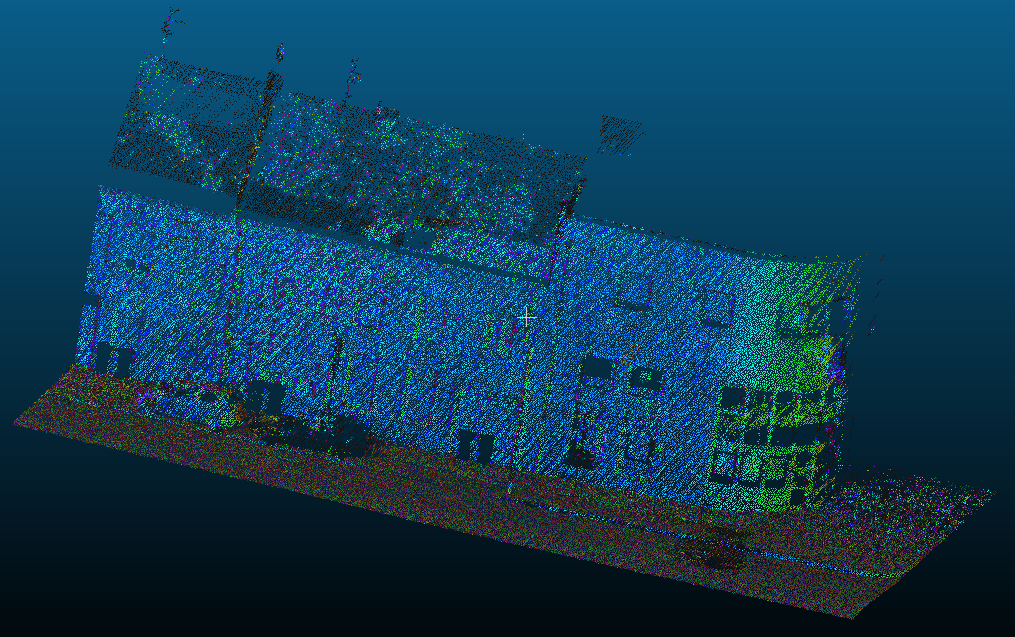
\includegraphics[width=0.483\textwidth]{small_radius.png}
	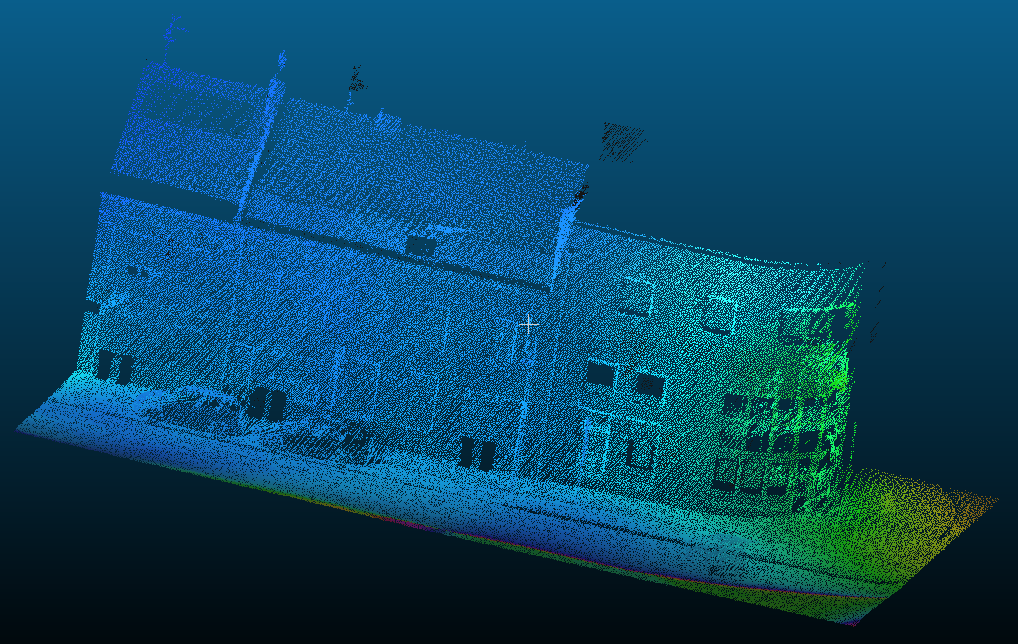
\includegraphics[width=0.48\textwidth]{huge_radius.png}
	\caption{Scalar field of normals computed and visualized with CloudCompare. Left: $r = 0.1$. Right: $r = 10$.}
	\label{fig:radius}
\end{figure}

\paragraph{Question 2}

TODO

\paragraph{Question 3} % ok

Figure \ref{fig:normals} shows the normals computed as a scalar field.

\begin{figure}[h!]
	\centering
	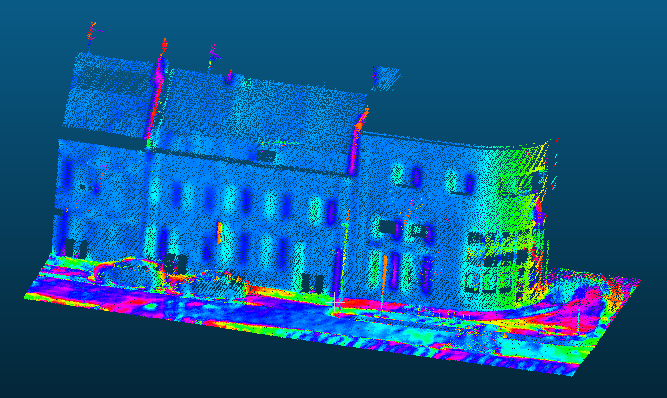
\includegraphics[width=0.7\textwidth]{lille_normals.png}
	\caption{TODO}
	\label{fig:normals}
\end{figure}

\paragraph{Question 4}

TODO

\paragraph{Question 5} % ok

All those classifiers take values in $[0,1]$ since $\lambda_1 \geq \lambda_2 \geq \lambda_3 \geq 0$.

In the case of a linear structure,  points almost belong to a line which is colinear to the eigenvector associated to $\lambda_1$, and one has $\lambda_1 \gg \lambda_2, \lambda_3$. Therefore, \emph{linearity} is high in that case.

Similarly, in the case of a solid surface, points belong to a 2D plane whose eigenvectors corresponding to $\lambda_1$ and $\lambda_2$ are a basis. In that case, $\lambda_1, \lambda_2 \gg \lambda_3$ and \emph{planarity} is close to 1.

Finally, in the case of scattered points, one has $\lambda_1 \approx \lambda_2 \approx \lambda_3$ and no dominant direction can be found. Hence \emph{sphericity} is high in that case.

The representation of these features on Lille point cloud as a scalar field in CloudCompare is given in figure \ref{fig:features}.

\begin{figure}[h!]
	\centering
	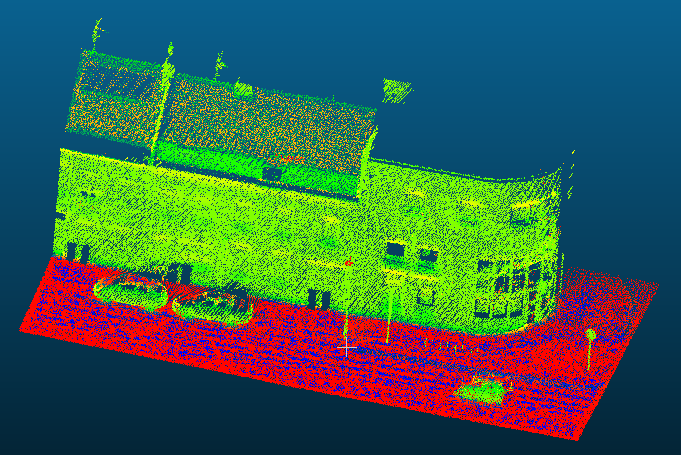
\includegraphics[width=0.56\textwidth]{verticality.png}
	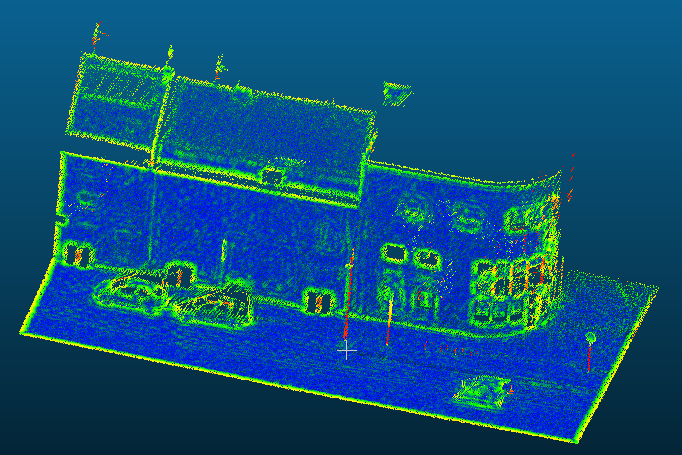
\includegraphics[width=0.56\textwidth]{linearity.png}
	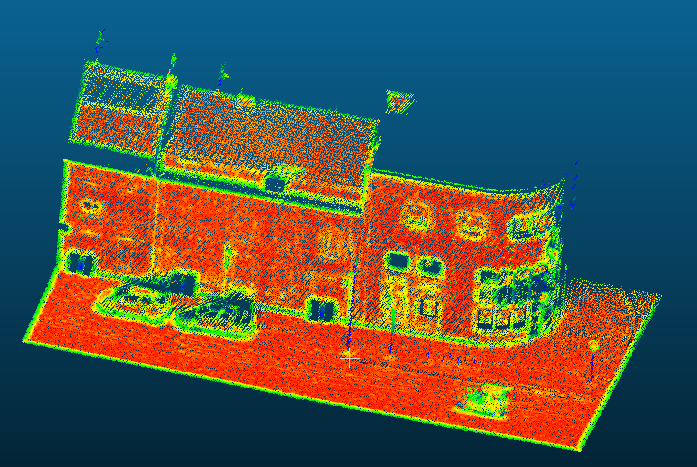
\includegraphics[width=0.56\textwidth]{planarity.png}
	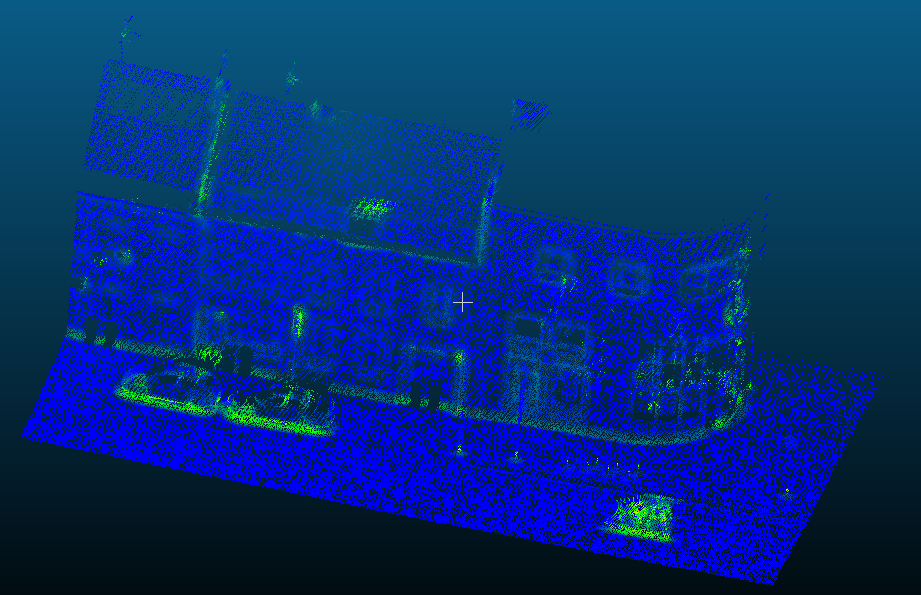
\includegraphics[width=0.56\textwidth]{sphericity.png}
	\caption{Computed features represented as scalar fields in CloudCompare. From top to bottom: verticality, linearity, planarity, sphericity}
	\label{fig:features}
\end{figure}



\end{document}